\begin{spacing}{1}
    \chapter*{Abstract}
\end{spacing}
\begin{wrapfigure}{r}{0.3\textwidth}
    \begin{center}
      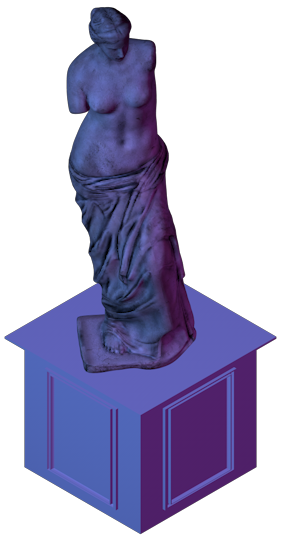
\includegraphics[width=0.2\textwidth]{pics/statue.png}
    \end{center}
\end{wrapfigure}
\setauthor{Litzlbauer Lorenz}
3D Portfolio Gallery is a web application developed by Ema Halilovic, Lorenz Litzlbauer and Fabian Maar as part of their thesis. The 3D Portfolio Gallery aims to enable designers to share their design portfolio with the world in an innovative way, all in a virtual three-dimensional space. 

Designers can use 3D Portfolio Gallery to create a three-dimensional portfolio from their own media (film, photo or 3D data). The 3D Portfolio Gallery offers a simple configuration process by selecting from a variety of exhibition rooms. Then the exhibition pieces can be placed there manually or automatically and supplied with additional information.
Those interested can move freely through the three-dimensional web exhibition and view the exhibits with different types of interaction.

The following applications were used for the implementation: Angular is used in the front end for the SPA (single-page application) logic and ThreeJs for the 3D presentation. The server uses technologies such as Quarkus, Maven, JPA, Panach and Hibernate ORM. To ensure the safety of users, we use JWT (JsonWebToken)

\newpage
\begin{spacing}{1}
    \chapter*{Zusammenfassung}
\end{spacing}
\begin{wrapfigure}{r}{0.3\textwidth}
    \begin{center}
      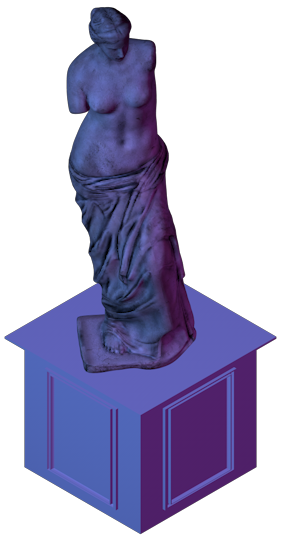
\includegraphics[width=0.2\textwidth]{pics/statue.png}
    \end{center}
\end{wrapfigure}
\setauthor{Litzlbauer Lorenz}
3D Portfolio Gallery ist eine Webapplikation, Lorenz Litzlbauer und Fabian Maar im Rahmen der Diplomarbeit entwickelt wurde. 3D Portfolio Gallery will Designer*innen ermöglichen, ihr Design-Portfolio auf eine innovative Art und Weise mit der Welt zu teilen und das alles in einem virtuellen dreidimensionalen Raum. Die Designer*innen können mithilfe von 3D Portfolio Gallery aus eigenen Medien (Film, Foto oder 3D-Daten) ein dreidimensionales Portfolio erstellen.
3D Portfolio Gallery wird als eine SPA im Web angeboten und ist über einen Web-Link erreichbar.
3D Portfolio Gallery bietet dafür einen einfachen Konfigurationsprozess, indem aus mehreren vordefinierten Grundrissen eine Gallery ausgewählt wird. In einem weiteren Schritt werden die Ausstellungsstücke entweder automatisch oder manuell platziert und mit Zusatzinformationen versehen.


Für die Umsetzung im Frontend werden folgende Frameworks verwendet: Angular für die SPA (Single-Page-Applikation) und ThreeJs für die 3D-Darstellung. . In der Frontend-Zugriffkontrolle und -Useridentifikation im Browser wird JWT (JsonWebToken) verwendet. Das JWT ist Teil eines Standards, der durch die III \href{https://www.rfc-editor.org/rfc/rfc7519}{RFC7519} IETF beschrieben wird.
Das Backend verwendet als Serverplattform Quarks, als Buildsystem Maven und in der Datenbankzugriffschicht JPA (Java Persistence Architecture), Panach und Hibernate ORM
